% Section content template for individual Educative lessons
% This file contains the actual content for a specific section
% Generated from Educative API section content

% Section: Getting Ready: Parking Lot
% Section ID: 6276164341727232
% Section Slug: getting-ready-parking-lot
% Generated: 2025-12-11T13:39:03.685944

\subsection{Problem definition}\label{KfyitG1dioESlbYIcgWus-1}
\\
A \textbf{parking lot} is a designated area for parking vehicles, commonly found in venues like shopping malls, sports stadiums, and office buildings. It consists of a fixed number of parking spots allocated for different types of vehicles. Each spot is charged based on the duration a vehicle remains parked. Parking time is tracked using a parking ticket issued at the entrance. Upon exit, the customer can pay using either an automated exit panel or through a parking agent, with a credit/debit card or cash as accepted payment methods.
\\
In this LLD interview case study, you'll focus on:

\begin{itemize}
\item
\protect\phantomsection\label{yKo5kkWCCclz2DMPMu8qg}
Managing parking for various vehicle types (car, van, truck, motorcycle, etc.) across potentially multiple floors and zones.
\item
\protect\phantomsection\label{w0W_Soz8xt7NCBeXSLmMm}
Allocating and tracking parking spot availability by type (e.g., compact, large, accessible, motorcycle).
\item
\protect\phantomsection\label{g42ZJeCg28JXv8R_3FX2-}
Issuing and managing parking tickets for tracking entry, parking duration, and exit.
\item
\protect\phantomsection\label{uzG47MSOrJadbThSLC6IS}
Handling flexible payments at automated exit panels or via human agents, supporting multiple payment methods (cash, card, coupon).
\item
\protect\phantomsection\label{7QXjk0bdZLSOag3_NSk1d}
Implementing and enforcing pricing models that may vary by hour, spot type, or vehicle type.
\item
\protect\phantomsection\label{EgWvX-XlnnRswya-WWOA1}
Ensuring real-time tracking of spot occupancy and enabling efficient entry/exit flows, especially during busy periods.
\item
\protect\phantomsection\label{uGMc3KzQhzuWbhiZu5mZA}
Accommodating special considerations like accessible parking spots and overflow situations.
\end{itemize}
\\
This parking lot system model can be adapted for various venues (malls, stadiums, offices, airports) and is extensible to different business rules (such as prebooking, dynamic pricing, or loyalty programs).

\begin{figure}[htbp]
 \centering
 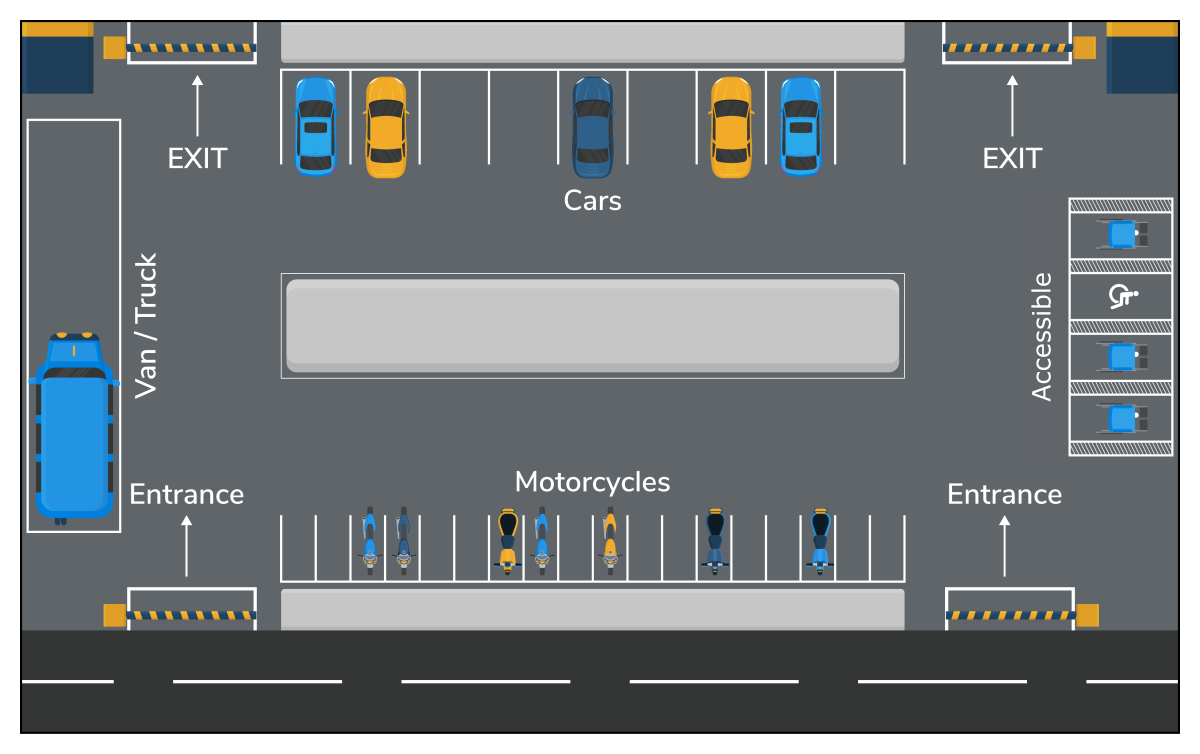
\includegraphics[width=0.5\textwidth]{Images/chapter_7/section_6276164341727232/5499599672180736.png}
 \caption{The layout of the parking lot}
\end{figure}

\subsection{Expectations from the interviewee}\label{KfyitG1dioESlbYIcgWus-2}
\\
A typical parking lot system has several components, each with specific constraints and requirements. The following section provides an overview of some major expectations the interviewer will want an interviewee to discuss in more detail.

\subsubsection{Payment flexibility}\label{GZ2teRz1DsKir8HY_5gOq}
\\
One of the most significant attributes of the parking lot system is the payment structure that it provides to its customers. An interviewer would expect you to ask questions like these:

\begin{itemize}
\item
\protect\phantomsection\label{zgi7KCvvwuw71T20blPzz}
How can customers pay at different exit points (i.e., at the automated exit panel or to the parking agent) and by different methods (cash, credit, or coupon)?
\item
\protect\phantomsection\label{dFY2CaLGWjQ-ja9mLNdws}
If the parking lot has multiple floors, how will the system keep track of customers who have already paid on a particular floor rather than at the exit?
\end{itemize}

\subsubsection{Parking spot type}\label{nzS_pSyYdqYgX-HzSpyaF}
\\
Another topic of discussion that an interviewer would expect you to be aware of is the different parking spot types (accessible, compact, large, and motorcycle), regarding which you can ask the following questions:

\begin{itemize}
\item
\protect\phantomsection\label{sUZ_IbKTxKNVUQi2LkWPX}
How will the parking capacity of each lot be considered?
\item
\protect\phantomsection\label{eVXwaCciGoR4B-UeyXlGD}
What happens when a lot becomes full?
\item
\protect\phantomsection\label{auT4XxkUofim8iRts2mTy}
How can one keep track of the free parking spots on each floor if there are multiple floors in the parking lot?
\item
\protect\phantomsection\label{xLWHGY-faAd9cKahr80YE}
How will the parking spots be divided among the four parking spot types in the lot?
\end{itemize}

\subsubsection{Vehicle types}\label{E2go_RGAjFJvVrqGzF2qa}
\\
Similar to the parking spot, an interviewer would also expect you to discuss the different vehicle types (car, truck, van, motorcycle), which can have the following set of questions:

\begin{itemize}
\item
\protect\phantomsection\label{bf7pctKaOHrstA781q5Tn}
How will capacity be allocated for different vehicle types?
\item
\protect\phantomsection\label{6x-fMJDXhzKZf8AoimpO4}
If the parking spot of any vehicle type is booked, can a vehicle of another type park in the designated parking spot?
\end{itemize}

\subsubsection{Pricing}\label{lNeaT5Umh8NpGnTsflMWm}
\\
We touched upon the payment structure offered by the parking lot system. Now , the pricing model needs to be clarified by the interviewer, and therefore, you may ask questions like these:

\begin{itemize}
\item
\protect\phantomsection\label{IEXZ_0HU3Gjal2USeqzeS}
How will pricing be handled? Should we accommodate having different rates for each hour? (For example, customers will have to pay \protect\phantomsection\label{katex_inline_qaWTXXRl7F34GrZ4i_pdI}{{{\( \$4 \)}}} for the first hour, \protect\phantomsection\label{katex_inline_Ryh-q_yCVKbYVIeE5Fr34}{{{\( \$3.5 \)}}} for the second and third hours, and \protect\phantomsection\label{katex_inline_D3Tb-1EZFaNNYCDONq789}{{{\( \$2.5 \)}}} for all the subsequent hours.)
\item
\protect\phantomsection\label{JBQ-5HwBs5QH7DAsLx34c}
Will the pricing be the same for the different vehicle types?
\end{itemize}

\subsection{Design approach}\label{cUH86ZMD2is391rK05pCi}
\\
We will design this parking lot system using a bottom-up design approach. For this purpose, we will follow the steps below:

\begin{itemize}
\item
\protect\phantomsection\label{XPEjY3rHekZwU69nb4nlI}
First, we'll identify the core entities such as \texttt{Vehicle}, \texttt{ParkingSpot}, \texttt{ParkingTicket}, and \texttt{Payment}, and define their primary responsibilities.
\item
\protect\phantomsection\label{1CD8z7GqPZIQ-ymn3WuAp}
Next, we'll model how vehicles are assigned to appropriate parking spots based on type and availability, how entry/exit is managed, and how parking duration is tracked.
\item
\protect\phantomsection\label{VMxYKEIAhyqCjDKBov965}
We'll design the system to support different payment methods and flexible pricing rules, ensuring secure and accurate fee calculation.
\item
\protect\phantomsection\label{7yQxCM1nFOwfF2SaJRR7a}
We'll ensure the system supports scalability (multiple floors, high traffic), real-time updates on availability, and follows SOLID principles for maintainability.
\end{itemize}
\\
Diagrams and code will illustrate the main workflows and class structures, discussed later in this case study.

\subsection{Design pattern~}\label{pCaGYU8B78ti-aCh2WyPC}
\\
During an interview, discussing the design patterns that a parking lot system falls under is always a good practice. Stating the design patterns gives the interviewer a positive impression and shows that the interviewee is well-versed in the advanced concepts of object-oriented design.
\\
Try to answer the following question. If you are not familiar with design patterns, don't worry! You can learn about them by asking, ``Define design patterns.''

\textbf{Question:}

Which design pattern(s) should be used to solve the problem of efficiently managing a parking lot? Explain your choice(s).

Let's explore the requirements of the parking lot system in the next lesson.

% End of section content